% File name: report/report.tex

\documentclass[a4paper,11pt]{article}  % Standard document class
\usepackage[english]{babel}            % Set document language
\usepackage{fullpage}                  % Set up page for small margins etc
\usepackage{listings}
\usepackage{graphicx}                  % For including images in document

\usepackage{tikz}
\usetikzlibrary{shapes,arrows}
%\usepackage{placeins}                  % Allows use of \FloatBarrier
% to avoid images or tables
% moving into next section
%\usepackage{subfig}                    % For subfigures...

\usepackage{amsmath}                   % For improving maths/formula typesetting
%\usepackage{tabularx}                  % Table changing package

%\usepackage{algpseudocode}             % For producing algorithms/flowcharts

\usepackage{listings}                  % For including source code in document
\lstset{
  basicstyle = \small
}

% Provide command for scientific notation
\providecommand{\e}[1]{\ensuremath{\times10^{#1}}}
\providecommand{\degrees}{\ensuremath{^{\circ}}}

% Define title here:
\title{4th Year Project: Soldering Machine}
\author{James Glanville}
\date{11th June 2013}

\begin{document}

% generate title
\maketitle

\section{Existing Solutions}
There are a number of hobbyist solutions to deal with SMD parts:

\begin{itemize}
	\item	Solder paste + heat:
		\begin{itemize}
			\item	Solder stencils: Expensive setup costs, very quick to use. Not suitable for
				this project due to cost.
			\item	Manual solder paste application: Mostly expensive dispenser, or with a syringe.
					Requires high accuracy while placing paste and is time consuming.
			\item	Hot air gun: Can be relatively difficult to get the right temperature profile.
			\item	Converted toaster over: seems quite common.
		\end{itemize}

	\item	Soldering by hand:
		\begin{itemize}
			\item	Dragging a bead of solder along pins, then cleaning up with solder sucker/wick.
				This requires a lot of feedback, which seems difficult to automate.
			\item	Some devices (SOIC?) have slightly bendy pins. A small amount of downwards 
				pressure on the pin onto a tinned pad can work, but this method will not work for leadless packages.
		\end{itemize}
\end{itemize}

\section{Project Idea}
I have decided to approach the project by building a machine which can place solder paste accurately, and then place
the surface mount devices on top. It should achieve this with minimal human interaction. The machine should also be able to
drill holes for through-hole devices, as well as be equiped with a milling bit for isolation routing through copper-clad pcbs.

\parskip 0.18in

When finished, the machine should be able to be connected to a computer via a USB port. A custom GUI will load the necessary 
design files (for example the holes to be drilled, pads to be soldered), generate the necessary GCODE, and send it to the printer.

\section{Requirements}

\subsection{X/Y axes}
A device pitch of 0.4mm (distance from centre of one pin to the next) is on the lower end of SMD ICs. Using solder paste,
devices will shift slightly upon heating to self-align. A requirement is that the device should be placed to a
small fraction of its pitch, so there is no danger of incorrect connections. I have decided to aim for an accuracy of +-0.05mm
in placement. This should be sufficient, but may be difficult to achieve in practice.

\subsection{Board size}
A maximum board size of 100x100mm would be sufficient for the vast majority of boards. I have chosen 100x100mm because that
is the maximum board size using the free version of EAGLE, a popular design package. As a result, there are a lot of designs
that use the maximum size, and it would be useful if this project allowed those designs to be populated.

\section{Design}

\subsection{X/Y axes}

The X/Y axes have the same requirements: +-0.05mm accuracy. There is the choice between moving the various tools over a stationary
bed, or keeping the tools stationary and moving the bed. I have decided to move only the bed, because it means that the pick
and place functionality does not have to move the parts, simply lift and lower them. This should reduce the risk of the parts
shifting on the needle, or falling off. It also allows for the use of more tools since weight is no longer a concern.

The bed will need travel distances of at least 100mm in both directions so that the entire bed can be accessed by tools. However,
there should also be space to place devices before they are automatically placed. This should need no more than 20-30mm in one axis
direction only.

Possible driving mechanisms:

\begin{itemize}
	\item	Toothed belts + pulleys + stepper motors: Simple, as used in reprap 3d printers. Can be run open loop
		very easily. The toothed belts stretch under load, and for the milling/drilling functionality are likely to deflect too much under loading.
		Requires: stepper motor + driver, belt, pulley.
	\item	Threaded rod + stepper motors: Cheap, slower but probably fast enough. M3-5 easy to couple
		to motor shafts (http://www.thingiverse.com/thing:9622).
	\item	Closed loop: dc motors + feedback. Linear potentiometers: relatively expensive, and potential
		issues with electrical noise. Rotary encoders: cheap, accurate (m4 pitch is ~0.5mm, not much
		travel/turn, might only need 10 slot encoder)

\end{itemize}

I have decided to utilise M6 threaded rod coupled to small stepper motors.

Linear slides:

\begin{itemize}
	\item	Drawer slides: cheap, surprisingly high precision.
	\item	3d printed bushings + steel rod. If 3d printer existance assumed, then very cheap solution.
	\item	LM8UUs (or smaller): About 50p each, relatively simple to use.
\end{itemize}

I have decided to use LM8UU bearings with steel rod. 

Motor selection:

Having chosen to use small stepper motors to control the axes, the choice of stepper motor is now important. I had
some NEMA17 motors, which claim a 2.2Kg/cm holding torque. I decided to run some tests to see what the maximum
speed I could run them at without skipping steps, and found a result of 8mm/s. This is sufficient for use in the
project (where speed is not a great concern), but I felt it would not be beneficial to use a smaller motor. 

\subsection{Z axis}
The Z axis will not require as much precision as the X and Y. Potential mechanisms:

\begin{itemize}
	\item	Micro servos: cheap (£2 on ebay). Require no drivers, and simple to drive. Z axis potentially
		does not need to be linear (UP/DOWN only?) so rotary-\textgreater linear mechanism simpler. If not linear,
		then hinging out of the way is a cheaper mechanism than slides.
\end{itemize}

\subsection{Part placement}

\begin{itemize}
	\item	Manual placement. Much more of a problem for a large number of SMD resistors/capacitors etc, than
		larger components. 
	\item	Vacuum "tweezers". Mechanically relatively simple, but problems of intelligent control, as well
		as well as storing the components before placement. As an experiment, I tried using an aquarium pump
		in reverse (by attaching the silicone tubing to the inlet instead of the outlet) connected to a fairly
		large diameter needle (ID: Xmm).
\end{itemize}

\subsection{Heated Bed}
Soldering to a hot board is easier (smaller temperature difference). This is now irrelevant as I shall not be soldering pin-by-pin.

\subsection{Flux application}
Solder paste includes flux, so this does not need an extra step. This is a useful consequence of using solder paste as opposed to solder,
where it would involve an additional placement step

\subsection{Drilling and isolation routing}
Isolation routing is a method to mill traces from copper-clad pcb. A conical engraving bit is used to cut very narrow tracks through
the copper, to leave disconnected pads as required. 

Drilling holes in pcbs is a time-consuming process to do by hand. If this machine could drill the holes automatically,
it would reduce the total time taken significantly. A small brushless motor with a collet would be enough. The biggest challenge
will be mechanically coupling the motor to the drill bit. This is not intrinsically difficult, but it should be made in a way that
is accessable to people without the use of a lathe (?)

A 25 Amp ESC (Turnigy plush 25A, £9) powering a small brushless motor (Turnigy 2217 20turn 860kv 22A outrunner, £10) is capable of milling
steel easily, so smaller, cheaper motors should be fine for routing/drilling copper.

The imodela cnc appears to use a small ball bearing for the shaft, with custom machined shafts. The milling bits fit inside the shaft, and
are secured with a single grub screw. This seems to work, though it would need a very carefully machined shaft so that axial misalignment
did not shear the end of the milling bit.

An alternative design would be to use a low cost rotary tool, which already has the bearings, collet and spindle motor. 

\subsection{Soldering iron}
Designing a mount for a cheap and widely available soldering iron may well have been the simplest approach. However, using solder paste, 
this part of the design is not needed.

\subsection{Melting solder paste}
Once the board has been pasted and the parts deposited, the solder paste needs to be heated up so that it will melt and form good connections.
There are a few possibilities for this process:

\begin{itemize} \itemsep0em
	\item	Oven: a small oven can be used to heat the entire board (see: http://www.openhardware.net/Misc\_Stuff/ToasterSMD/). This appears to
			work well, however the oven should not be used for food after that, since the components of solder paste are toxic. As a result,
			it can be an expensive method since it requires dedicated, expensive hardware.
	\item	Hand-held hot air gun: A small hot air gun can be used to gradually melt the solder for the components. There is a requirement
			for the hot air gun that it emits sufficiently hot air at a sufficiently low velocity that the solder will melt, but also that
			the devices will not shift under the force. I use a hot air attachment with a butane-powered soldering iron which works nicely.
			This does require the most human interaction (since it is less likely that the flow of hot air will cover the board uniformly, but it
			is not a particularly precise process.
	\item	Hot-plate. A small hot-plate can be used to heat the board from underneath (see http://www.hobbytronics.co.uk/hotplate-smd-soldering).
			An advantage compared to the oven method is that a piece of thermally conductive metal can be used between a hotplate and the board, so
			that the hot plate will not become food-unsafe. 
\end{itemize}
			
The choice of method to heat the solder paste may well depend on the end-user - one solution is not clearly superior to the others. During the
course of this project I am likely to use the hand-held hot air gun since I possess the equipment.

\subsection{Electronics/Firmware}
I have decided to use an avr chip to translate GCODE to stepper motor commands for the following reasons:
\begin{itemize} \itemsep0em
	\item	Cost: an atmega328 is £2-3, a usb-serial chip is <£2, which is not much.
	\item	Mature open source firmware (GRBL, https://github.com/grbl/grbl) is available for gcode-\textgreater stepper
		conversion, which leaves more time to focus on other parts of this project.
\end{itemize}

On the host pc, custom software will have to be written to translate the design into a gcode file to be sent to the machine. Usefully however,
the machine's firmware will not need to be written or modified.

\section{Serial interface}
For simplicity, the communication between the PC and the electronics board is implemented as a serial link. An arbitrary baud rate of 57600 has been
chosen, this is sufficiently fast so that the electronics board is not slowed by waiting for instructions (as the firmware buffers incoming commands in
a small buffer in RAM), and sufficiently slow that the error rate is assumed to be zero.

\subsection{USB-serial cable}
A usb-serial cable based on the FTDI ft232r chipset can be plugged into the serial header on the electronics board. This is a cheap (<£5) device that is 
a complete solution. Driver support for the FT232R is available for all platforms that have been considered (Windows/OSX/Linux/Android).

\subsection{Bluetooth serial link}
\begin{figure}[ht!]
\centering
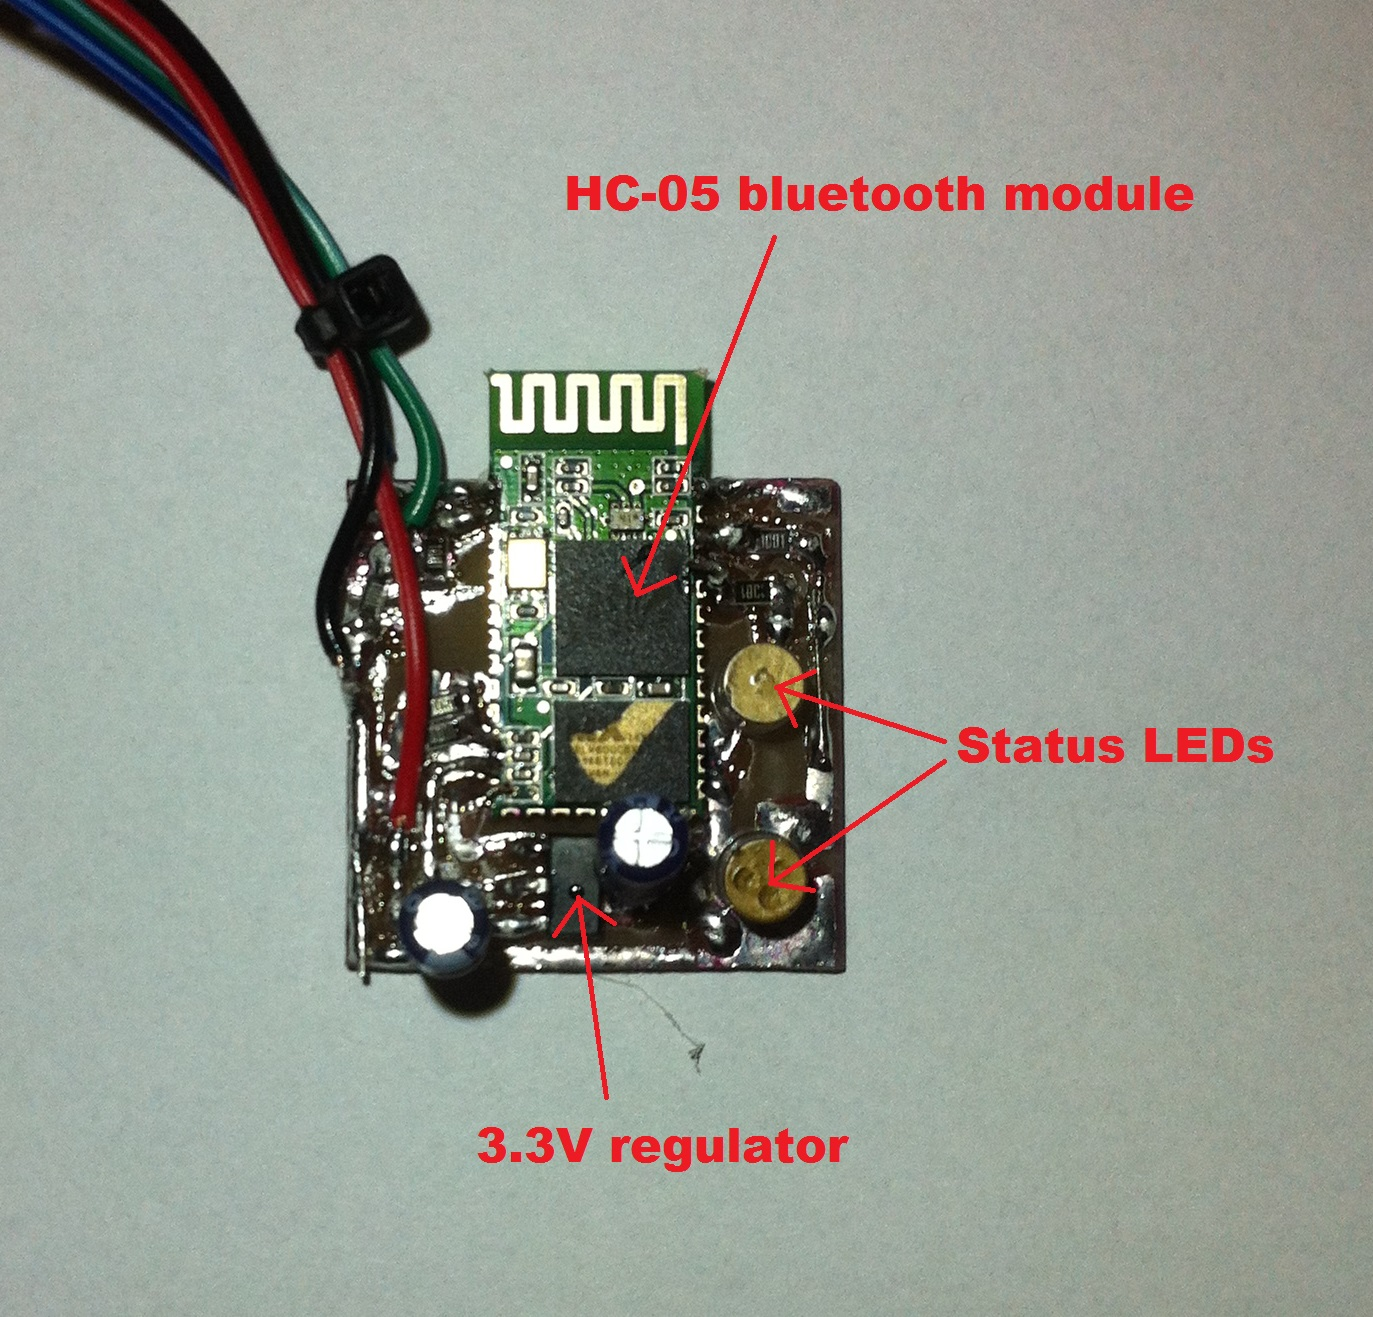
\includegraphics[width=90mm]{resources/bluetoothmodule.jpg}
\caption{Bluetooth module mounted on breakout board.}
\label{overflow}
\end{figure}

As an alternative to a USB-serial cable, a bluetooth link can be used. Depending on the end user, this may be more convenient. The HC-05 bluetooth module was
chosen because of its low cost (£3.50) and simplicity. The board requires a 3.3V supply, which is not present on the electronics board. I made a small
breakout board for the module, including an AMS1117-3.3 3.3V linear regulator (£0.10) and link status LEDs. The 3.3V TX output from the module is sufficient
for the AVR despite its higher 5V supply. To avoid damage to the bluetooth module, a potential divider consisting of two 1k resistors is used. This 2.5V output is
again sufficient for the bluetooth module.

To configure the baud rate for the bluetooth module, it was connected to a pc using a usb-serial cable. The bluetooth module is powered up whilst the "KEY" pin is held high (3.3V).
This starts the module in AT configuration mode. The baud rate was then set by sending the string "AT+UART=57600,1,0" at 38400 baud. This configuration is only required once,
the module stores all configuration in non-volatile storage.

\section{Host computer software}
Software will have to be written to translate board cad data to gcode. Some of this already exists in the public domain, some will have to be made
as part of this project.

Isolation milling and drilling: pcb2gcode (https://github.com/festlv/pcb2gcode-metric). Takes gerber designs and generates isolation routing/drilling
gcode. It is also capable of voronai isolation (functionally equivalent routing that cuts the least amount of material). The only configuration
will be to generate a millproject file with the correct cutting depths.

Solder paste placement: No freely available software (as far as I am aware).

Device placement: No freely available software (as far as I am aware).

The solder paste placement should be relatively straightforward. The program will simply need to find the locations of the pads, calculate their
area, and then apply a suitable amount of paste to them. For ICs, the paste will not need to be separately applied to each pin (due to the high
surface tension of molten solder), so some method of detecting ICs on the board layout will be needed.

The code to place devices will be the most challenging. However, provided there is a sensible area in which to hand-deposit the devices, it should
not be too hard to calculate how to transport them to the required location.

In my opinion, the most challenging part of writing the conversion code will simply be to extract the necessary data from the cad files. Once this
has been obtained, the gcode should be easy to create.

\section{Tools}
I have a small mill, a 3d printer and a lathe. It may be worth considering that a lot of people/schools have
access to a laser cutter and perhaps mill/lathe, so if possible all custom components could be 3d printed or 
lasercut.

\section{Solder paste extrusion}
I have decided to use the design here: http://www.thingiverse.com/thing:20733

The extruder works by applying pressure to the top of the solder paste syringe. Pressure is applied by tightening a pulley made
of T5 timing belt with a geared stepper motor. I chose this design because the extruder is compact, and the design allows for
fast reduction of pressure, important for clean extrusion and to avoid the solder paste dribbling. 

To calibrate the extruder, two parameters are needed: steps/volume extruded and retraction steps. The first is easy to calculate:

(All dimensions in mm,mm\textsuperscript{2},mm\textsuperscript{3})
\begin{align}
	Volume extruded per step &= (cross-sectional area of syringe * T5 pitch * number of teeth of T5 pulley) \\&/ (number of microsteps/step * steps/rotation of motor * gear reduction ratio)\\
	&= (66.1276*5*10)/(16*200*12)\\
	&= 0.0861 mm\textsuperscript{3}\\
\end{align}

\begin{align}					 
	Steps/mm\textsuperscript{3} &= 1 / volume extruded per step\\
	&= 1 / 0.0861\\
	&= 11.61\\
\end{align}

The retraction steps must be experimentally determined. The choice is a tradeoff between minimising solder paste dribble (large number
of retraction steps) and reducing total process time (small number of retraction steps). It must be enough that negligible pressure is
exerted on the syringe when retracted.

Some method to "prime" the extruder will be needed. Assuming the extruder is initially hand-tightened so that the belt has little slack,
a possible method is to repeatedly advance the extruder and then retract by a slightly smaller amount, until the user notifies the machine
that solder paste has been extruded. At this point, the extruder should pause after retracting. The solder paste deposition process can
then commence since the exact point of extrusion has been established. Assuming that x is the required granularity of calibration (the 
maximum amount of solder paste that will be wasted), and y is the retraction distance, the following example gcode will carry out this calibration:

\begin{lstlisting}[frame=single]
//values in braces {} are to be evaluated on the host

//Start loop here:
G92 E{y} //Set extruder position in firmware to be y
G1 E{x+y} //Extrude x amount of paste
G1 E{y} //Retract
//if user has not indicated extrusion then loop again

//when the user has indicated extrusion:
G92 E{y}
\end{lstlisting}
	  
\section{Managing devices prior to placement}
There will need to be a way to place the devices in a known position, so they can then be picked up and placed in their final locations.
Commercial pick and place machines take the parts directly from the reels they are supplied in. While this is optimal for that application in that
it is a very fast way to operate, the cost of reel dispensers is prohibitive for this machine. Instead, the parts will have to be roughly placed
by hand. There are a number of ways this could be done:

\begin{itemize} \itemsep0em
	\item	Embossed outlines of all necessary device footprints.
	\item	Rectangular embossed outline, devices to be located in one corner.
\end{itemize}

I have decided that the latter will be easiest to implement. A rectangular hole will be milled into the bed. Each part can then
be manually placed inside, then pushed to one corner. A consistent system will be needed to ensure correct orientation. I have decided to use
the following set of rules:

\begin{itemize} \itemsep0em
	\item	ICs will be placed with pin1 touching the datum corner.
	\item	Devices will always be placed with the longest side (if applicable) touching the long side of the rectangle.
	\item	Devices such as mosfets will be placed with the corner between the longest side and side with most pins touching the datum corner.
	\item	Polar 2-lead devices with always have the anode nearest the datum corner.
\end{itemize}

Given the current component to be placed, and the device footprint, it will be trivial to find the coordinates of the centre of the part. Some
consideration will have to be given as to how to determine the centre of mass of parts which are not symmetrical in two directions (eg mosfets).
	   
\section{Vacuum Placing}
\subsection{Prototype}
To test how effectively small parts could be placed with a vacuum, I made a simple test setup:

\begin{itemize} \itemsep0em
	\item	12V diaphragm air pump (£8.89 - ebay)
	\item	6mm OD/4mm ID silicone tube (£2.69/m - ebay)
	\item	various needles (need more info here)
	\item	MOSFET
	\item	330$\Omega$ resistor
\end{itemize}

\begin{figure}[ht!]
\centering
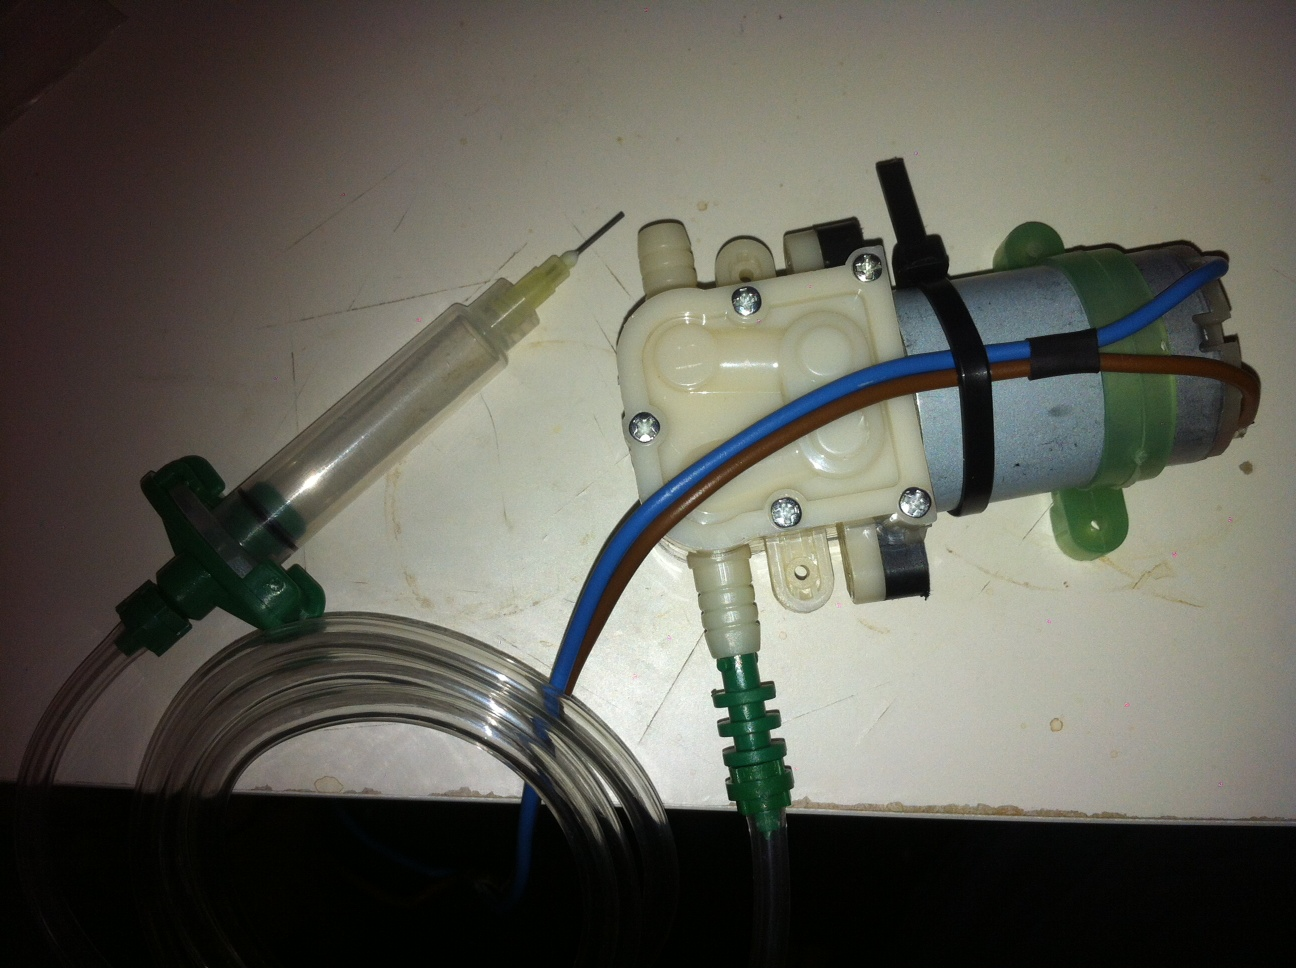
\includegraphics[width=90mm]{resources/pump_and_hose.jpg}
\caption{Pump with hose and needle.}
\label{hose and needle}
\end{figure}

The pump draws ~200mA at 12V, which is easily controlled with a MOSFET. Using a 1.8mm ID needle, SOIC-20 parts were picked up, 
and had significant friction against the needle - essential to avoid slipping or rotating. It was important to place the needle 
as centrally as possible on the part to avoid generating any imbalance that allowed the part to fall. 

\subsection{Conclusions}
A vacuum needle solution is workable, and a good choice for this project. Things that need to be considered for use in the final project:

\begin{itemize}
	\item	The pump takes a certain time to generate a vacuum because of the relatively large internal volume of the pump
		and silicon tube. It will be important to measure this, and add a margin of error so that full suction is applied
		to each device before any movement takes place. Similarly, when turning off the pump, the pressure must return to
		atmospheric before the device can be considered to have been placed succesfully. In testing, the pump I used took
		less than a second to leak sufficiently for this to occur, but if another pump were to be used, it may be necessary
		to place a tiny hole in the air line so that pressure drops quickly.
	\item	It is important to place the needle very near to the centre of mass of the device. The majority of devices will be
		symmetrical, which will make this easier.
	\item	The needle must be able to be raised and lowered to the correct heights. It may be possible to push the needle down
		with a weak spring, with a micro servo that raises it - this would remove any need to know the exact height of each
		device. This will need to be tested.
\end{itemize}

\begin{figure}[ht!]
\centering
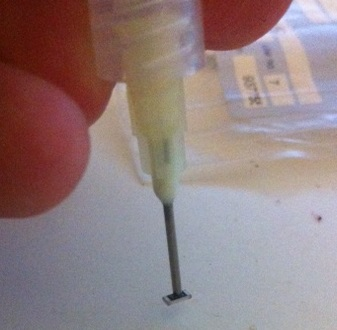
\includegraphics[width=90mm]{resources/needle_with_resistor.jpg}
\caption{SMD resistor being picked up.}
\label{overflow}
\end{figure}

\section{Measuring Accuracy}
It is important to measure the accuracy of the axes to ensure that they can reach the specified +-0.05mm. This will need to be measured
at all points on the bed (as the accuracy will worsen when the bed is central due to increased rod deflection.). Of particular concern will be
the deflection under the load of the isolation routing bit. The solder paste and device placement will not involve any significant force. The 
drilling will generate a force, but the tolerance required of a 1mm hole is not nearly as demanding as that of the isolation routing cutter.
I have not yet measured the exact forces exerted by the routing bit, but I estimate that they are 5-10N. This means that the anti-backlash nut
will need to exert the same or greater force to ensure that the board does not move. This in turn places extra resistance on the motor movement.

\section{Operating Steps}

% Define block styles
\tikzstyle{decision} = [diamond, draw, fill=blue!20, 
    text width=4.5em, text badly centered, node distance=3cm, inner sep=0pt]
\tikzstyle{block} = [rectangle, draw, fill=blue!20, 
    text width=14em, text centered, rounded corners, minimum height=3em]
\tikzstyle{line} = [draw, -latex']
\tikzstyle{cloud} = [draw, ellipse,fill=red!20, node distance=7cm,
    minimum height=2em]
    
\begin{tikzpicture}[align=center,node distance = 1.6cm,auto]
    % Place nodes
    \node [block] (pcb2gcode) {run pcb2gcode to generate GCODE};
    \node [cloud, left of=pcb2gcode, align=center] (designfiles) {PCB designs exported\\ from design package\\ in GERBER format};
    
    \node [block, below of=pcb2gcode] (isolationinit) {attach spindle, load isolation milling bit, zero};
    \node [block, below of=isolationinit] (isolation) {send routing GCODE to machine};
    \node [block, below of=isolation, fill=orange!70] (isolationcheck) {visually check board for errors};
    
    \node [block, below of=isolationcheck] (drillinit) {load drill bit, zero};
    \node [block, below of=drillinit] (drill) {send drilling GCODE to machine};
    \node [block, below of=drill, fill=orange!70] (drillcheck) {visually check board for errors};
    
    \node [block, below of=drillcheck] (pasteinit) {load paste extruder};
    \node [block, below of=pasteinit] (paste) {send solder paste GCODE to machine};
    \node [block, below of=paste, fill=orange!70] (pastecheck) {visually check board for errors};
    
    \node [block, below of=pastecheck] (vacuuminit) {load vacuum needle};
    \node [block, below of=vacuuminit] (vacuum) {send pick and place GCODE to machine};
    \node [block, below of=vacuum, fill=orange!70] (vacuumcheck) {visually check board for errors};
    
    \node [block, below of=vacuumcheck] (reflow) {Heat board to melt solder paste};
    % Draw edges
    \path [line,dashed] (designfiles) -- (pcb2gcode);
    \path [line] (pcb2gcode) -- (isolationinit);
    \path [line] (isolationinit) -- (isolation);
    \path [line] (isolation) -- (isolationcheck);
    \path [line] (isolationcheck) -- (drillinit);
    \path [line] (drillinit) -- (drill);
    \path [line] (drill) -- (drillcheck);
    \path [line] (drillcheck) -- (pasteinit);
    \path [line] (pasteinit) -- (paste);
    \path [line] (paste) -- (pastecheck);
    \path [line] (pastecheck) -- (vacuuminit);
    \path [line] (vacuuminit) -- (vacuum);
    \path [line] (vacuum) -- (vacuumcheck);

    \path [line] (vacuumcheck) -- (reflow);
 %   \path [line] (isolation) -- (isolationcheck);
 %   \path [line] (isolationcheck) -- (drillinit);

\end{tikzpicture}

\section{Building pcb2gcode from source in windows}

get pcb2gcode source:
git clone git@github.com:JamesGlanville/pcb2gcode-metric.git

install VS 2012 PRO

Download \begin{verbatim}http://ftp.gnome.org/pub/gnome/binaries/win32/gtk+/2.24/gtk+-bundle_2.24.10-20120208_win32.zip
from http://www.gtk.org/download/win32.php
place in pcbgcode-metric folder

download gerbv from http://sourceforge.net/projects/gerbv/
gerbvinst-2.6.1.exe and install

download boost_1_55_0.zip from http://sourceforge.net/projects/boost/
unzip contents to c:\\boost155
open VS2012 x86 Native Tools Command Prompt, from C:\\ProgramData\\Microsoft\\Windows\\Start Menu\\Programs\\Microsoft Visual Studio 2012\\Visual Studio Tools
AS ADMINISTRATOR
cd c:\\boost155
bootstrap.bat
bjam.exe

download http://ftp.gnome.org/pub/GNOME/binaries/win32/gtkmm/2.22/gtkmm-win32-devel-2.22.0-2.exe
from http://ftp.gnome.org/pub/GNOME/binaries/win32/gtkmm/2.22/
and install.

download gerbv-2.6.1.tar.gz from http://sourceforge.net/projects/gerbv/files/gerbv/gerbv-2.6.1/
and extract to c:\\gerbv-2.6.1

hack appwindow.c
create config.h
create demo-config.h
\end{verbatim}

\end{document}
